% vim: set spell spelllang=en tw=100 et sw=4 sts=4 foldmethod=marker foldmarker={{{,}}} :

\documentclass{beamer}

\usepackage{tikz}
\usepackage{xcolor}
\usepackage{complexity}
\usepackage{hyperref}
\usepackage{microtype}
\usepackage[vlined]{algorithm2e} % algorithms

\usetikzlibrary{shapes, arrows, shadows, calc, positioning, fit}
\usetikzlibrary{decorations.pathreplacing, decorations.pathmorphing, shapes.misc}
\usetikzlibrary{tikzmark}

\colorlet{screenverylightgrey}{black!2!white}
\colorlet{screengrey}{black!30!white}

\definecolor{uofgblue}{rgb}{0, 0.321569, 0.533333}
\colorlet{uofgblue20}{uofgblue!20!white}
\colorlet{uofgblue40}{uofgblue!40!white}
\colorlet{uofgblue60}{uofgblue!60!white}
\colorlet{uofgblue80}{uofgblue!80!white}

\definecolor{uofgstone}{rgb}{0.498039, 0.454902, 0.403922}

\definecolor{uofgtdarkgreen}{rgb}{0.380392, 0.564706, 0.501961}
\definecolor{uofgtlightgreen}{rgb}{0.615686, 0.788235, 0.729412}
\definecolor{uofgtyellow}{rgb}{0.85098, 0.827451, 0.643137}
\definecolor{uofgtorange}{rgb}{0.784314, 0.694118, 0.545098}

% {{{ theme things
\useoutertheme[footline=authorinstitutetitle]{miniframes}
\useinnertheme{rectangles}

\setbeamerfont{block title}{size={}}
\setbeamercolor*{structure}{fg=uofgblue}
\setbeamercolor*{palette primary}{use=structure,fg=black,bg=white}
\setbeamercolor*{palette secondary}{use=structure,fg=black,bg=uofgblue40}
\setbeamercolor*{palette tertiary}{use=structure,fg=white,bg=uofgblue}
\setbeamercolor*{palette quaternary}{fg=white,bg=black}

\setbeamercolor*{titlelike}{parent=palette primary}

\beamertemplatenavigationsymbolsempty

\tikzset{vertex/.style={draw, circle, inner sep=0pt, minimum size=0.5cm, font=\small\bfseries}}
\tikzset{notvertex/.style={vertex, color=white, text=black}}
\tikzset{plainvertex/.style={vertex}}
\tikzset{selectedvertex/.style={vertex, fill=uofgblue}}
\tikzset{vertexc1/.style={vertex, fill=uofgblue40}}
\tikzset{vertexc2/.style={vertex, fill=uofgblue}}
\tikzset{vertexc3/.style={vertex, fill=uofgtdarkgreen}}
\tikzset{vertexc4/.style={vertex, fill=uofgtorange}}
\tikzset{edge/.style={color=screengrey}}
\tikzset{bedge/.style={ultra thick}}
\tikzset{edgel1/.style={ultra thick, color=uofgblue}}
\tikzset{edgel2/.style={ultra thick, color=uofgblue40}}
\tikzset{edgel3/.style={ultra thick, color=uofgtdarkgreen}}
\tikzset{edgel4/.style={ultra thick, color=uofgtorange}}

\setbeamertemplate{title page}
{
    \vbox{}
    \vspace*{0.5cm}
    \begin{center}
        {\usebeamerfont{title}\inserttitle\par}
        \vskip0.5cm\par
        \begin{beamercolorbox}[sep=8pt,center]{author}
            \usebeamerfont{author}\insertauthor
        \end{beamercolorbox}
        {\usebeamercolor[fg]{titlegraphic}\inserttitlegraphic\par}
    \end{center}
    \vfill

    \begin{tikzpicture}[remember picture, overlay]
        \node at (current page.north west) {\begin{tikzpicture}[remember picture, overlay]\fill
        [fill=uofgblue, anchor=north west] (0, 0) rectangle (\paperwidth, -1.5cm);\end{tikzpicture}};
        \node [anchor=north west, shift={(0.2cm,-0.2cm)}] at (current page.north west) {\includegraphics*[keepaspectratio=true,scale=0.5]{UoG_keyline.eps}};
    \end{tikzpicture}
}

% }}}

\title{Russian Doll Search}
\author[Ciaran McCreesh]{\textcolor{uofgblue}{Ciaran McCreesh}}

\begin{document}

{
    \usebackgroundtemplate{\includegraphics*[keepaspectratio=true, height=\paperheight]{background.jpg}}
    \begin{frame}[plain]
        \titlepage
    \end{frame}
}

\begin{frame}{An Old Maximum Clique Algorithm}

    \only<1>{
        \centering
        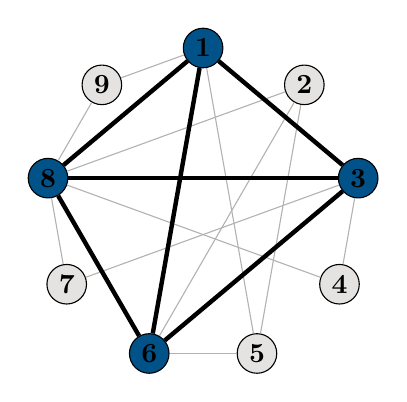
\begin{tikzpicture}%{{{
            \newcount \c
            \foreach \n in {1, ..., 9}{
                \c=\n
                \multiply\c by -40
                \advance\c by 130
                \ifthenelse{\n = 1 \OR \n = 3 \OR \n = 6 \OR \n = 8}{
                    \node[draw, circle, fill=uofgblue, inner sep=2pt] (N\n) at (\the\c:2) {\textbf{\n}};
                }{
                    \node[draw, circle, fill=uofgstone!20!white, inner sep=2pt] (N\n) at (\the\c:2) {\textbf{\n}};
                }
            }

            \draw [edge] (N1) -- (N5); \draw [edge] (N1) -- (N9);
            \draw [edge] (N2) -- (N5); \draw [edge] (N2) -- (N6); \draw [edge] (N2) -- (N8);
            \draw [edge] (N3) -- (N4); \draw [edge] (N3) -- (N7);
            \draw [edge] (N4) -- (N8);
            \draw [edge] (N5) -- (N6);
            \draw [edge] (N7) -- (N8);
            \draw [edge] (N8) -- (N9);

            \draw [bedge] (N1) -- (N3);
            \draw [bedge] (N6) -- (N8);
            \draw [bedge] (N1) -- (N6);
            \draw [bedge] (N1) -- (N8);
            \draw [bedge] (N3) -- (N6);
            \draw [bedge] (N3) -- (N8);
        \end{tikzpicture}%}}}
        \\~
    }

    \only<2>{
        \begin{center}
            \includegraphics*[keepaspectratio=true,scale=0.2]{ostergard-paper.png}
        \end{center}
    }

    \only<3>{
        \begin{itemize}
            \item Let $G[V']$ be the subgraph of $G$ induced by $V'$
                \begin{itemize}
                    \item The subgraph with some of the vertices, and all of the edges between those vertices.
                \end{itemize}

            \item Let $V' + w$ mean $V' \cup \{ w \}$, with the assertion that $w \notin V'$.

            \item Let $\omega(G)$ be the size of a maximum clique in $G$.

            \item Now $\omega(G[V' + w])$ is either $\omega(G[V'])$ or $\omega(G[V']) + 1$.
                \begin{itemize}
                    \item And if the latter, it must contain $w$.
                \end{itemize}
        \end{itemize}
    }

    \only<4>{
        \begin{itemize}
            \item Write out the vertices of a graph in some static order, $v_1, v_2, \ldots, v_n$.

            \item Let $V_i$ be the vertices $\{ v_i, v_{i + 1}, \ldots, v_n \}$.

            \item $\omega(G[V_n])$ is $1$.

            \item $\omega(G[V_i])$ is either $\omega(G[V_{i + 1}])$ or $\omega(G[V_{i + 1}]) + 1$.
                \begin{itemize}
                    \item And if the latter, it must contain $v_i$.
                \end{itemize}

            \item $\omega(G)$ is $\omega(G[V_1])$.

            \item So we find $\omega(G[V_n])$, then $\omega(G[V_{n - 1}])$, and so on, down to
                $\omega(G[V_1]) = \omega(G)$.
        \end{itemize}
    }

    \only<5>{
        \begin{itemize}
            \item We grow cliques recursively: $C$ is our growing clique, and $P$ is the undecided
                vertices which can be added to $C$.

            \item We pick a vertex $v$, add it to $C$, and remove from $P$ any vertex not adjacent
                to $v$. Then we recurse until $P$ is empty, and then backtrack and pick a new $v$.
        \end{itemize}
    }

    \only<6>{
        \begin{itemize}
            \item Now the clever bit: if $j$ is the lowest-numbered vertex left in $P$, then
                $\omega(G[V_j])$ gives us a bound on how much further we can extend the growing
                clique.

                \begin{itemize}
                    \item And $j > i$, thanks to the static variable ordering: $P$ initially contains
                        only vertices to the right of our top-level $i$.
                \end{itemize}

            \item This is a better bound than $|P|$, because it knows about relationships between
                undecided vertices.
        \end{itemize}

        \begin{center}
            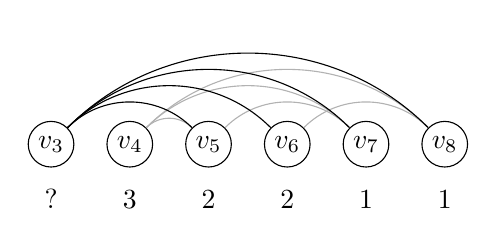
\begin{tikzpicture}%{{{
                \node (V3) [draw, circle, inner sep = 2pt] at (0, 0) { $v_3$ };
                \node (V4) [draw, circle, inner sep = 2pt] at (1, 0) { $v_4$ };
                \node (V5) [draw, circle, inner sep = 2pt] at (2, 0) { $v_5$ };
                \node (V6) [draw, circle, inner sep = 2pt] at (3, 0) { $v_6$ };
                \node (V7) [draw, circle, inner sep = 2pt] at (4, 0) { $v_7$ };
                \node (V8) [draw, circle, inner sep = 2pt] at (5, 0) { $v_8$ };

                \node at (0, -0.7) { $?$ };
                \node at (1, -0.7) { $3$ };
                \node at (2, -0.7) { $2$ };
                \node at (3, -0.7) { $2$ };
                \node at (4, -0.7) { $1$ };
                \node at (5, -0.7) { $1$ };

                \draw [color = screengrey] (V6) to [out = 45, in = 135] (V8);
                \draw [color = screengrey] (V5) to [out = 45, in = 135] (V7);
                \draw [color = screengrey] (V4) to [out = 45, in = 135] (V5);
                \draw [color = screengrey] (V4) to [out = 45, in = 135] (V7);
                \draw [color = screengrey] (V4) to [out = 45, in = 135] (V8);

                \draw (V3) to [out = 45, in = 135] (V5);
                \draw (V3) to [out = 45, in = 135] (V6);
                \draw (V3) to [out = 45, in = 135] (V7);
                \draw (V3) to [out = 45, in = 135] (V8);
            \end{tikzpicture}%}}}
        \end{center}
    }

\end{frame}

\begin{frame}{Valued Constraint Satisfaction Problems}

    \only<1>{
        \begin{itemize}
            \item A Valued Constraint Satisfaction Problem has a set of variables, a set of
                constraints, and a well-behaved way of assigning a cost to violating a subset of the
                constraints.

                \begin{itemize}
                    \item Flexible enough to handle Partial CSPs, Additive CSPs with hard
                        constraints, Probabilistic CSPs, \ldots
                    \end{itemize}

            \item We seek an assignment of values to variables which minimises this cost.
        \end{itemize}
    }

    \only<2>{
        \begin{itemize}
            \item One possible model for maximum clique:
                \begin{itemize}
                    \item A boolean variable $V_i$ for each vertex $v_i$, determining whether it is in the
                        clique.
                    \item For each pair of nonadjacent vertices $v_i$ and $v_j$, a constraint ``not
                        ($V_i$ and $V_j$)'', with cost infinity.
                    \item For each vertex, a constraint ``$V_i$ is true'', with cost 1.
                    \item The total cost is the sum of the cost of violated constraints, and tells us the
                        number of vertices \emph{not} in the clique.
            \end{itemize}
        \end{itemize}
    }

    \only<3>{
        \begin{itemize}
            \item A simple lower bound looks at violations in already-assigned variables (backward
                checking).
            \item Add up the costs of all of the constraints we've already violated.
            \item If the cost of the constraints we've violated so far is greater than or
                equal to the cost of the best solution we've found so far, we can backtrack
                immediately.
            \item For clique: how many vertices have we rejected so far?
        \end{itemize}
    }

    \only<4>{
        \begin{itemize}
            \item We can also look at constraints which have only one unassigned variable (forward
                checking).
            \item For each constraint with one uninstantiated variable, pick the value for that
                variable that has the cheapest cost. Now add these costs together.
            \item For clique: how many vertices can no longer be included?
        \end{itemize}
    }
\end{frame}

\begin{frame}{Russian Doll Search}
    \only<1>{
        \begin{center}
            \includegraphics*[keepaspectratio=true,scale=0.2]{dolls-paper.png}
        \end{center}
    }

    \only<2>{
        \begin{center}
            \includegraphics*[keepaspectratio=true,scale=0.4]{russiandolls.jpg}

            \vspace{2em}
            \tiny \url{http://commons.wikimedia.org/wiki/File:Russian-Matroshka2.jpg} (cropped), CC-BY-SA 3.0
        \end{center}
    }

    \only<3>{
        \begin{itemize}
            \item Write out the variables in some static order, $V_1, V_2, \ldots, V_n$.
            \item Solve the problem containing just $V_n$, and remember the cost.
            \item Solve the problem containing just $V_{n - 1}$ and $V_n$, using the static variable
                ordering, and remember the cost. If at any point the cost of a partial assignment
                plus the best cost of assigning $V_n$ (which we know) is more than the best so far,
                backtrack immediately.
            \item Now add $V_{n - 2}$ and solve.
            \item And so on, until we solve for all variables.
        \end{itemize}
    }

    \only<4>{
        \begin{itemize}
            \item Typically, the Russian dolls pass is used only once, at the top of search. After that,
                regular branch and bound is used.

            \item We could do Russian dolls at every level. But this is very expensive, and might not
                improve the bound by much.
        \end{itemize}
    }
\end{frame}

\begin{frame}{Where is it Used?}
    \only<1>{
        \begin{itemize}
            \item Seems to be good if we have a fairly well-behaved objective function, but a very
                weak bound.

                \begin{itemize}
                    \item Earth Observation Satellite Scheduling
                    \item Radio Link Frequency Assignment
                    \item DNA Analysis
                    \item Maximum Density Still-Life (until Chu and Stuckey solved it)
                \end{itemize}
        \end{itemize}
    }

    \only<2>{
        \begin{center}
            \includegraphics*[keepaspectratio=true,scale=0.4]{vaskelainen-paper.png}
        \end{center}

        \begin{itemize}
            \item Covering problems in directed graphs and hypergraphs:
                \begin{itemize}
                    \item Steiner triple
                    \item Maximum transitive subtournament
                    \item Best barbequeue
                \end{itemize}
        \end{itemize}
    }
\end{frame}

\begin{frame}{Pseudo-Tree Decompositions}
    \only<1>{
        \begin{center}
            \includegraphics*[keepaspectratio=true,scale=0.2]{larrosa-paper.png}
        \end{center}

        \vspace{2em}

        \begin{center}
            \includegraphics*[keepaspectratio=true,scale=0.5]{sanchez-paper.png}
        \end{center}
    }

    \only<2-3>{
        \begin{center}
            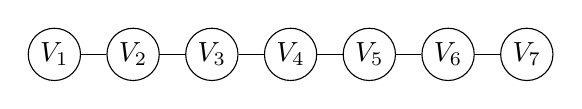
\begin{tikzpicture}%{{{
                \node (V1) [draw, circle, inner sep = 2pt] at (0, 0) { $V_1$ };
                \node (V2) [draw, circle, inner sep = 2pt] at (1, 0) { $V_2$ };
                \node (V3) [draw, circle, inner sep = 2pt] at (2, 0) { $V_3$ };
                \node (V4) [draw, circle, inner sep = 2pt] at (3, 0) { $V_4$ };
                \node (V5) [draw, circle, inner sep = 2pt] at (4, 0) { $V_5$ };
                \node (V6) [draw, circle, inner sep = 2pt] at (5, 0) { $V_6$ };
                \node (V7) [draw, circle, inner sep = 2pt] at (6, 0) { $V_7$ };

                \draw (V1) -- (V2);
                \draw (V2) -- (V3);
                \draw (V3) -- (V4);
                \draw (V4) -- (V5);
                \draw (V5) -- (V6);
                \draw (V6) -- (V7);
            \end{tikzpicture}%}}}
        \end{center}

        \vspace*{0.5cm}

        \begin{center}
            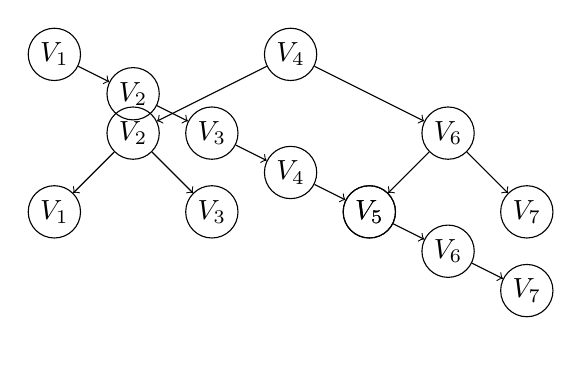
\begin{tikzpicture}%{{{
                \node <2> (V1) [draw, circle, inner sep = 2pt] at (0, -1) { $V_1$ };
                \node <2> (V2) [draw, circle, inner sep = 2pt] at (1, -1.5) { $V_2$ };
                \node <2> (V3) [draw, circle, inner sep = 2pt] at (2, -2) { $V_3$ };
                \node <2> (V4) [draw, circle, inner sep = 2pt] at (3, -2.5) { $V_4$ };
                \node <2> (V5) [draw, circle, inner sep = 2pt] at (4, -3) { $V_5$ };
                \node <2> (V6) [draw, circle, inner sep = 2pt] at (5, -3.5) { $V_6$ };
                \node <2> (V7) [draw, circle, inner sep = 2pt] at (6, -4) { $V_7$ };

                \draw <2> [arrows=->] (V1) -> (V2);
                \draw <2> [arrows=->] (V2) -> (V3);
                \draw <2> [arrows=->] (V3) -> (V4);
                \draw <2> [arrows=->] (V4) -> (V5);
                \draw <2> [arrows=->] (V5) -> (V6);
                \draw <2> [arrows=->] (V6) -> (V7);

                \node <3> (V1) [draw, circle, inner sep = 2pt] at (0, -3) { $V_1$ };
                \node <3> (V2) [draw, circle, inner sep = 2pt] at (1, -2) { $V_2$ };
                \node <3> (V3) [draw, circle, inner sep = 2pt] at (2, -3) { $V_3$ };
                \node <3> (V4) [draw, circle, inner sep = 2pt] at (3, -1) { $V_4$ };
                \node <3> (V5) [draw, circle, inner sep = 2pt] at (4, -3) { $V_5$ };
                \node <3> (V6) [draw, circle, inner sep = 2pt] at (5, -2) { $V_6$ };
                \node <3> (V7) [draw, circle, inner sep = 2pt] at (6, -3) { $V_7$ };

                \draw <3> [arrows=->] (V2) -> (V1);
                \draw <3> [arrows=->] (V2) -> (V3);
                \draw <3> [arrows=->] (V4) -> (V2);
                \draw <3> [arrows=->] (V4) -> (V6);
                \draw <3> [arrows=->] (V6) -> (V5);
                \draw <3> [arrows=->] (V6) -> (V7);

                \node at (6, -4.5) { ~ };
            \end{tikzpicture}%}}}
        \end{center}
    }

    \only<4>{
        \begin{center}
            \includegraphics*[keepaspectratio=true,scale=0.6]{kerning.png}

            \vspace{1em}
            \tiny \url{http://xkcd.com/1015/} (Randall Munroe), CC-BY-NC 2.5
        \end{center}
    }
\end{frame}

\begin{frame}{Specialisation}
    \only<1>{
        \begin{center}
            \includegraphics*[keepaspectratio=true,scale=0.2]{specialisation-paper.png}
        \end{center}

        \begin{itemize}
            \item Instead of looking at variables, look at variable-value pairs.
            \item This is even more expensive, but sometimes it pays off if we do it selectively.
        \end{itemize}
    }
\end{frame}

\begin{frame}{Elimination Rules}
    \begin{itemize}
        \item We can reduce the number of dolls using a greedy heuristic: we can move variables that
            may be added without increasing the cost to the left of our current variable, and skip
            the following iterations.
    \end{itemize}
\end{frame}

\begin{frame}{Parallelism?}
\end{frame}

\begin{frame}[b]
        \small
        \begin{semiverbatim}
17:31 < sdstrowes> you know the problem with russian dolls?
17:31 < sdstrowes> they're just so full of themselves.
        \end{semiverbatim}
    \vfill
    \begin{center}
    \url{http://dcs.gla.ac.uk/~ciaran} \\
    \href{mailto:c.mccreesh.1@research.gla.ac.uk}{\nolinkurl{c.mccreesh.1@research.gla.ac.uk}}
\end{center}
\begin{tikzpicture}[remember picture, overlay]
    \node at (current page.north west) {\begin{tikzpicture}[remember picture, overlay]\fill
    [fill=uofgblue, anchor=north west] (0, 0) rectangle (\paperwidth, -1.5cm);\end{tikzpicture}};
    \node [anchor=north west, shift={(0.2cm,-0.2cm)}] at (current page.north west) {\includegraphics*[keepaspectratio=true,scale=0.5]{UoG_keyline.eps}};
\end{tikzpicture}
\end{frame}

\end{document}

